\lecture{3: Birthday Problem, Properties of Probability}
\textbf{Key Topics:} Birthday problem, properties of probability, inclusion-exclusion

\subsection*{Lecture Summary}
\begin{itemize}
    \item Birthday problem that defies intuition
    \item Properties of probability given the axioms
    \item Inclusion-exclusion theorem and application
\end{itemize}

\subsection*{Birthday Problem}

There are $k$ people in a room. Assume each person’s birthday is equally likely to be any of the 365 days of the year (we exclude February 29), and that people’s birthdays are independent (we will define independence formally later, but intuitively it means that knowing some people’s birthdays gives us no information about other people’s birthdays; this would not hold if, e.g., we knew that two of the people were twins). What is the probability that at least one pair of people in the group have the same birthday?

If $k > 365$, by the pigeonhole principle, the probability is 1. Let $k\le 365$.

\begin{align*}
    &P(\text{no match}) = \frac{365\cdot364\cdots(365-k+1)}{365^k} \\
    \implies &P(match) \approx 
    \begin{cases}
        50.7 \%, & \text{if } k=23 \\
        97\%, & \text{if } k=50 \\
        99.99\%, & \text{if } k=100
    \end{cases}
\end{align*}

It’s surprising that even with a much smaller number of people it’s overwhelmingly likely that there is a birthday match. For a quick intuition into why it should not be so surprising, note that with 23 people there are $\binom{23}{2} = 253$ \textit{pairs} of people, any of which could be a birthday match.

\subsection*{Properties of Probability}

\theorem{\textbf{Properties of Probability} (\bookref{Ch. 1.6})\\
Probability has the following properties, for any events $A$ and $B$.
\begin{enumerate}[label=\arabic*.]
    \item $P(A^c) = 1 - P(A)$.
    \item If $A \subseteq B$, then $P(A) \le P(B)$.
    \item $P(A\cup B) = P(A) + P(B) - P(A\cap B)$.
\end{enumerate}
\textit{Proof.}
\begin{enumerate}[label=\arabic*.]
    \item Since $A$ and $A^c$ are disjoint and their union is $S$,
    $$
    1=P(S)=P(A\cup A^c) = P(A)+P(A^c)
    $$
    \item If $A \subseteq B$, then $B = A \cup (B\cap A^c)$, where $A$ and $(B\cap A^c)$ disjoint.
    $$
    P(B) = P(A) + P (B \cap A^c) \ge P(A)
    $$
    \item $P(A\cup B) = P(A \cup (B \cap A^c)) = P(A) + P(B \cap A^c)$. It suffices to show that $P(B \cap A^c) = P(B) - P(A\cap B)$, but we know that $B = (A \cap B) \cup (A^c \cap B)$ which are disjoint.
\end{enumerate}

}

The third property is a special case of \textit{inclusion-exclusion}, a formula for finding the probability of a union of events when the events are not necessarily disjoint. For three events, inclusion-exclusion says
\begin{align}
    P(A\cup B \cup C) = &P(A) + P(B) + P(C)\\
    &-P(A\cap B) - P(A \cap C) - P(B \cap C)\\
    &+P(A\cap B\cap C)
\end{align}

For intuition consider this Venn Diagram:
\begin{center}
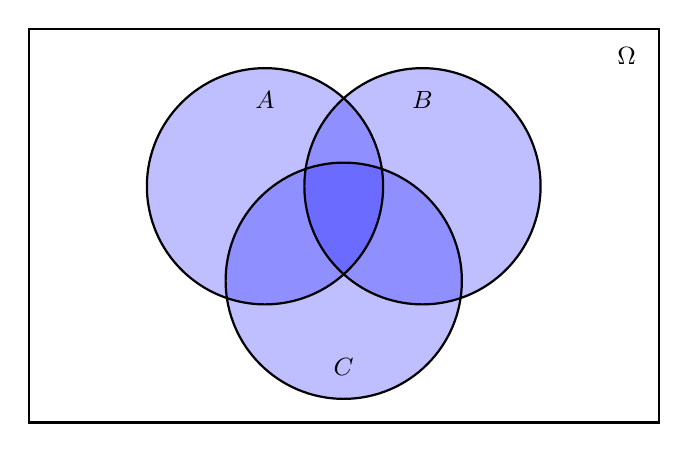
\begin{tikzpicture}[font=\small]
  % Parameters
  \def\W{8}   % rectangle width
  \def\H{5}   % rectangle height
  \def\r{1.5} % circle radius

  % Rectangle (sample space)
  \draw[thick] (0,0) rectangle (\W,\H) node[pos=0.98,below left] {$\Omega$};

  % Clip everything to the rectangle so circles stay inside
  \begin{scope}
    \clip (0,0) rectangle (\W,\H);

    % Fill the union by filling each circle with same color and opacity
    \fill[blue,opacity=0.25] (3.0,3.0) circle (\r); % A
    \fill[blue,opacity=0.25] (5.0,3.0) circle (\r); % B
    \fill[blue,opacity=0.25] (4.0,1.8) circle (\r); % C
  \end{scope}

  % Draw circle outlines and labels
  \draw[thick] (3.0,3.0) circle (\r) node[yshift=1.1cm] {$A$};
  \draw[thick] (5.0,3.0) circle (\r) node[yshift=1.1cm] {$B$};
  \draw[thick] (4.0,1.8) circle (\r) node[yshift=-1.1cm] {$C$};

  % Title / probability text
  %\node at (4,-0.5) {$P(A\cup B\cup C)$};

\end{tikzpicture}
\end{center}
To get the total area of the shaded region $A \cup B \cup C$, we start by adding the areas of the three circles, $P(A) + P(B) + P(C)$. The three football-shaped regions have each been counted twice, so we then subtract $P(A \cap B) + P(A \cap C) + P(B \cap C)$. Finally, the region in the center has been added three times and subtracted three times, so in order to count it exactly once, we must add it back again. This ensures that each region of the diagram has been counted once and exactly once

Now we can write inclusion-exclusion for $n$ events.

\theorem{\textbf{Inclusion-exclusion} (\bookref{Ch. 1.6})\\
For any events $A_1, \dots, A_n$,
\begin{align*}
    P\left( \bigcup^n_{i=1} A_i\right) = \sum_i P(A_i) - \sum_{i < j}P(A_i \cap A_j) + \sum_{i < j< k} P(A_i \cap A_j \cap A_k) -\dots\\
    +(-1)^{n+1} P(A_1 \cap \dots \cap A_n).
\end{align*}
}

This formula can be proven by induction using just the axioms, but instead we’ll present a shorter proof later on after introducing some additional tools. The rationale behind the alternating addition and subtraction in the general formula is analogous to the special cases we’ve already considered.

The next example, \textit{de Montmort’s matching problem}, is a famous application of inclusion-exclusion. Pierre Rémond de Montmort was a French mathematician who studied probability in the context of gambling and wrote a treatise devoted to the analysis of various card games. He posed the following problem in 1708, based on a card game called Treize.

\example{\textbf{de Montmort's matching problem}\\
Consider a well-shuffled deck of $n$ cards, labeled 1 through $n$. You flip over the cards one by one, saying the numbers 1 through $n$ as you do so. You win the game if, at some point, the number you say aloud is the same as the number on the card being flipped over (for example, if the 7th card in the deck has the label 7). What is the probability of winning?

Let $A_i$ be the event that the $i$th card in the deck has the number $i$ written on it. We are interested in the probability of the union $A_1 \cup \cdots \cup A_n$: as long as at least one of the cards has a number matching its position in the deck, you will win the game. First,
$$
P(A_i) = \frac{1}{n}.
$$
By symmetry: the card numbered $i$ is equally likely to be in any of the $n$ positions in the deck, so it has probability $1/n$ of being in the $i$th spot. Second,
$$
P(A_i \cap A_j) = \frac{(n-2)!}{n!} = \frac{1}{n(n-1)},
$$
since we require the cards numbered $i$ and $j$ to be in the $i$th and $j$th spots in the deck and allow the remaining $n-2$ cards to be in any order, so $(n-2)!$ out of $n!$ possibilities are favorable. Similarly,
$$
P(A_i \cap A_j \cap A_k) = \frac{1}{n(n-1)(n-2)}.
$$
In the inclusion-exclusion formula, there are $n$ terms involving one event, $\binom{n}{2}$ terms involving two events, $\binom{n}{3}$ terms involving three events, and so forth. By the symmetry of the problem, all $n$ terms of the form $P(A_i)$ are equal, all $\binom{n}{2}$ terms of the form $P(A_i \cap A_j)$ are equal, and the whole expression simplifies considerably:
\begin{align*}
    P\left( \bigcup^n_{i=1} A_i\right) &= n\cdot \frac{1}{n} - \binom{n}{2} \cdot \frac{1}{n(n-1)} + \binom{n}{3} \cdot \frac{1}{n(n-1)(n-2)} - \cdots + (-1)^{n+1} \cdot \frac{1}{n!}\\
    &= 1 - \frac{1}{2!} + \frac{1}{3!} - \cdots + (-1)^{n+1} \cdot \frac{1}{n!}\\
    &\approx 1 - \frac{1}{e}
\end{align*}
}